The HPS experiment is installed in the downstream alcove of experimental Hall B at Jefferson Lab as shown in Fig.~\ref{Figure:hallB}~\cite{beamline_nim_2017}. Due to the construction of the CLAS12 detector in Hall B as part of the 12~GeV upgrade, HPS running was planned for nights and weekends when running beam would not interfere with CLAS12 construction. After the partial failure of the CHL, HPS received dedicated, continuous running during May of 2015 in support of the Engineering Run. 

\begin{figure}[htb]
  \centering
      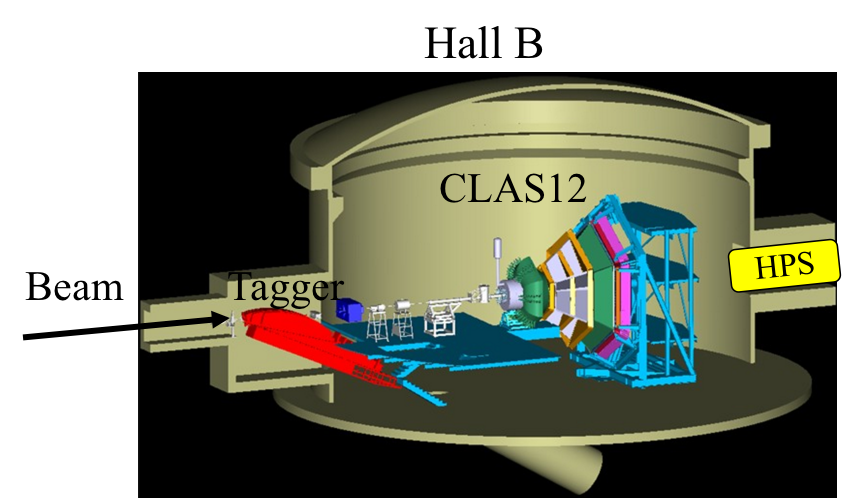
\includegraphics[width=0.6\textwidth]{pics/experiment/hallB.png}
  \caption[HPS location in Hall B]{The HPS experiment is in the downstream alcove of Hall B and ran while not interfering with CLAS12 construction.}
  \label{Figure:hallB}
\end{figure}

\begin{figure}[htb]
  \centering
      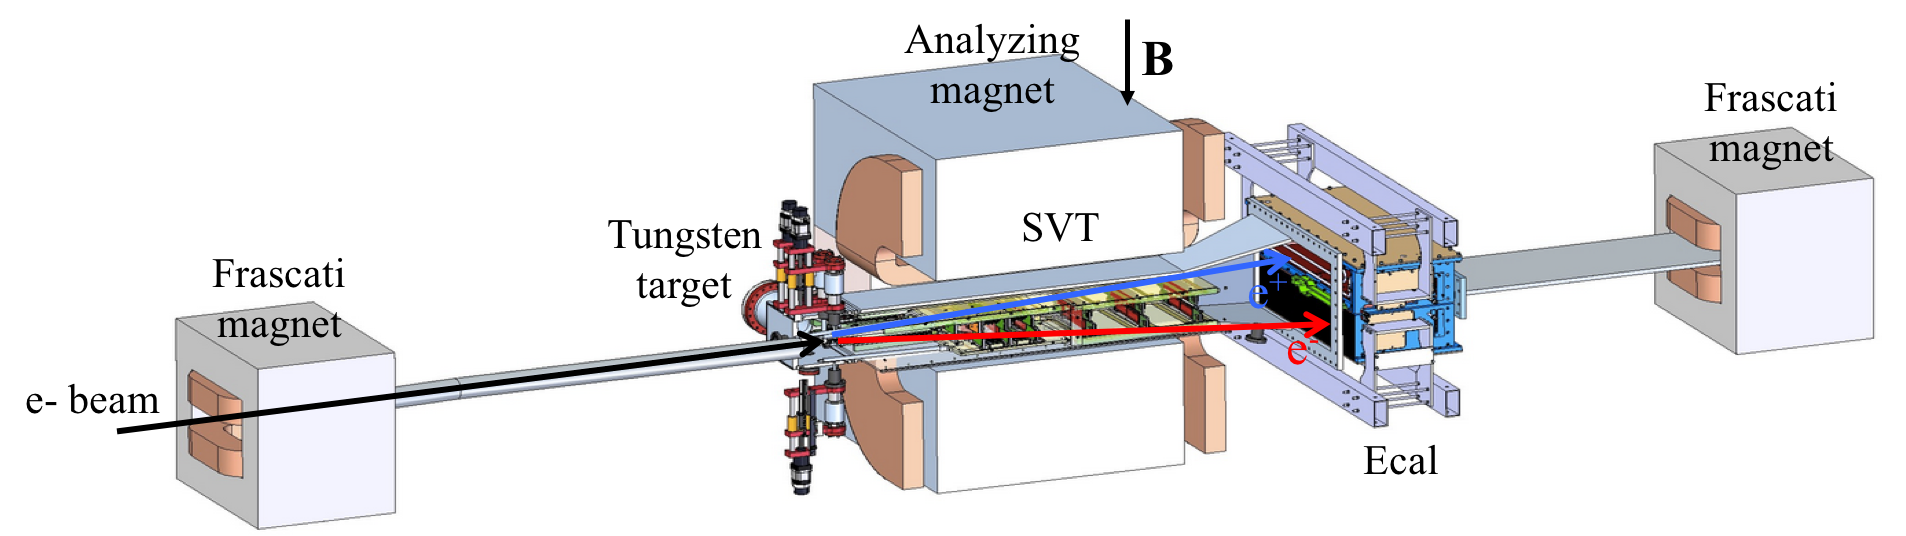
\includegraphics[width=1.0\textwidth]{pics/experiment/hpsBeamline.png}
  \caption[HPS beamline]{A drawing of the HPS experiment is shown. After the electron beam passes through Hall B and into the alcove, the beam enters the first Frascati magnet. The electron beam hits the tungsten target, located in the Pair Spectrometer magnet, at an angle of approximately 30.5~mrad. Particles created from the interaction of the beam at the target pass through the six tracking layers of the SVT before depositing their energy into the ECal.}
  \label{Figure:hpsBeamline}
\end{figure}

\begin{figure}[htb]
  \centering
      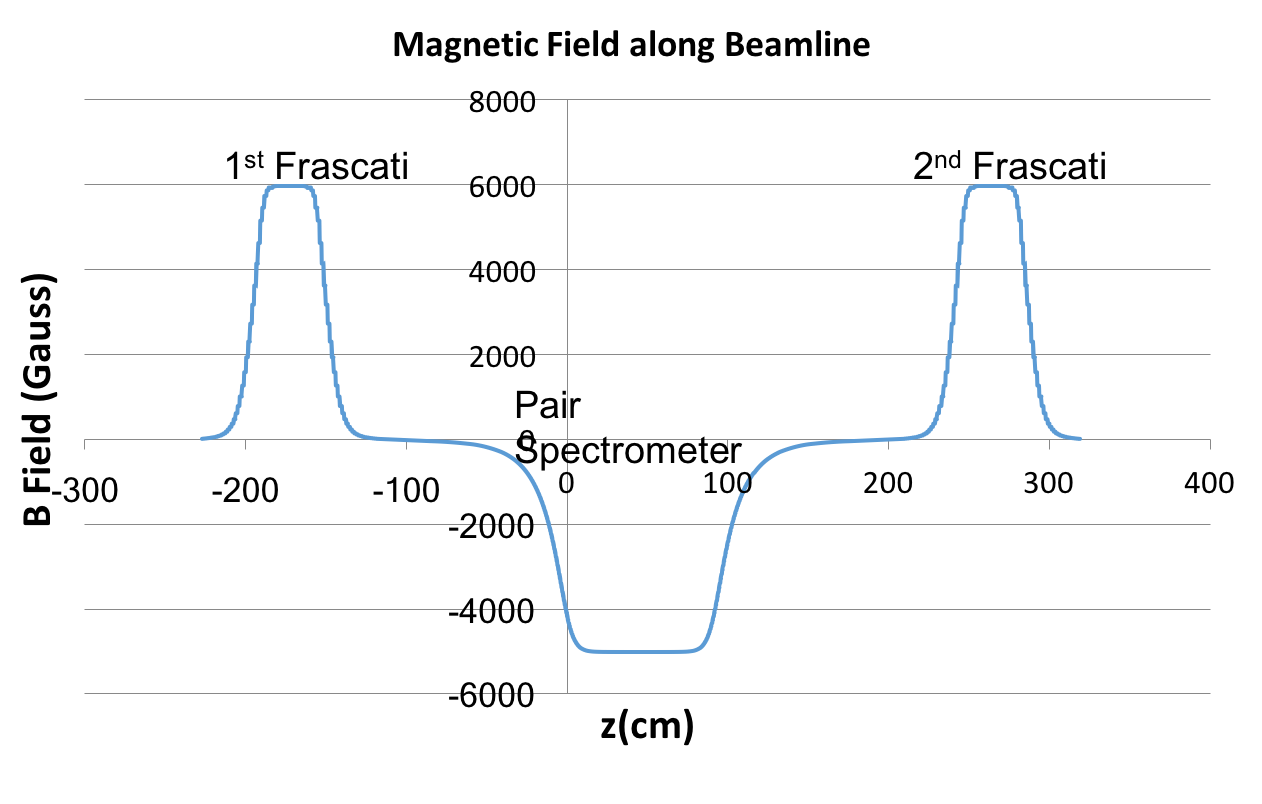
\includegraphics[width=1.0\textwidth]{pics/experiment/bfield.png}
  \caption[HPS magnetic fields]{The dipole magnetic field values for 2.2~GeV running where $z$ is the distance along the beamline from the target.}
  \label{Figure:bField}
\end{figure}

\begin{figure}[htb]
  \centering
      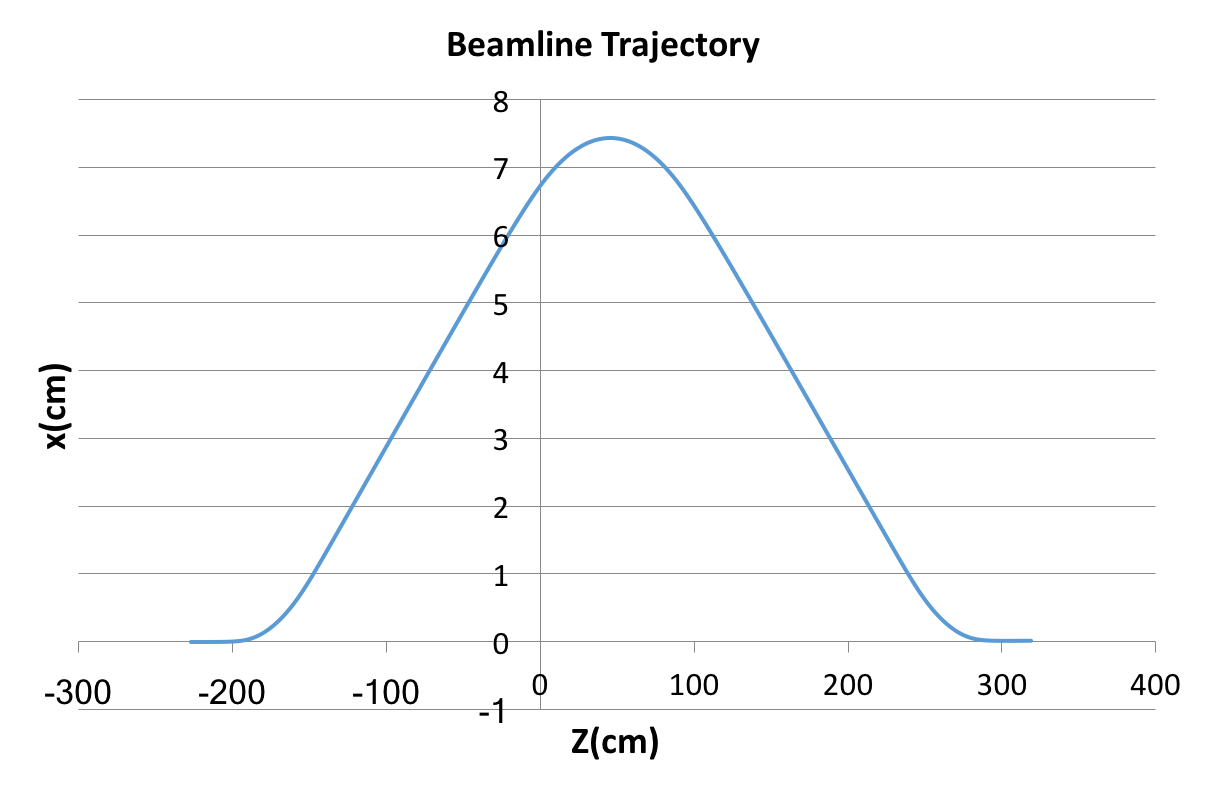
\includegraphics[width=1.0\textwidth]{pics/experiment/feetrajectory.png}
  \caption[Charged particle trajectory in HPS beamline]{The horizontal trajectory of a 2.2~GeV electron through the three dipole chicane along the beamline where $z$ is the distance along the beamline and $x$ is transverse to $z$. The target position is at $z=0$.}
  \label{Figure:trajectory}
\end{figure}

\begin{figure}[htb]
  \centering
      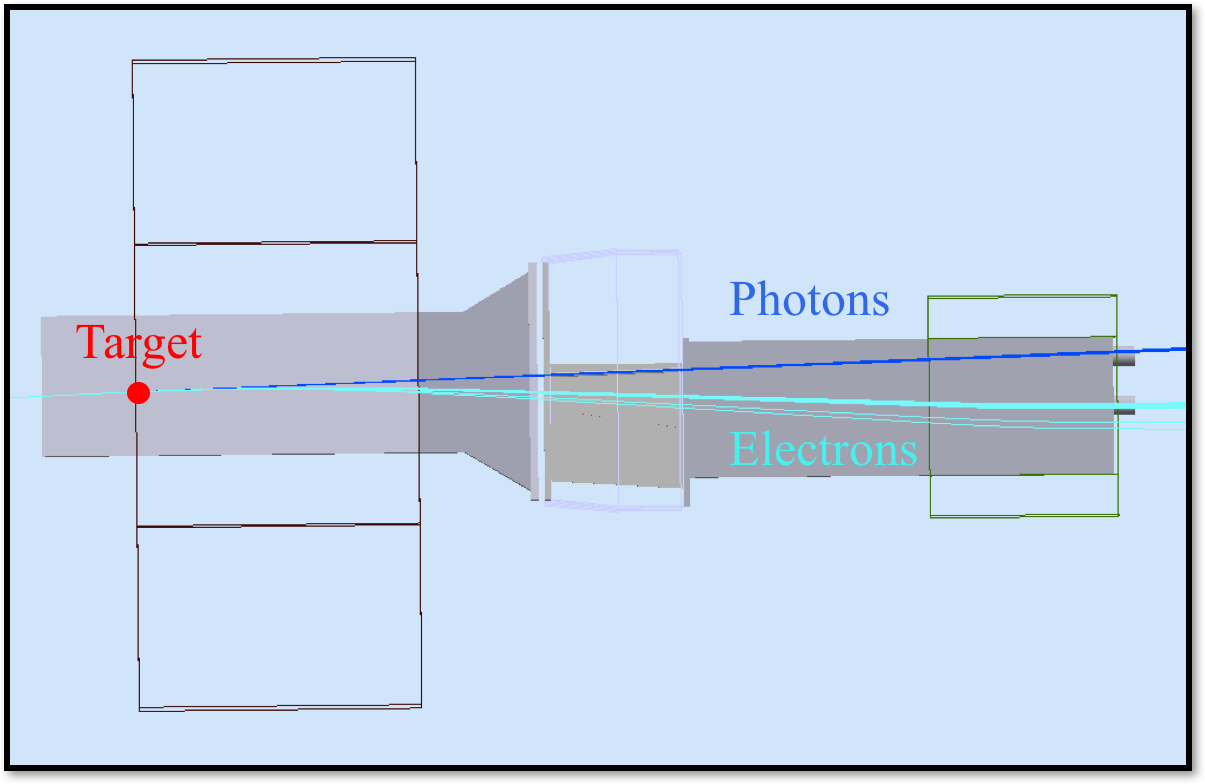
\includegraphics[width=0.8\textwidth]{pics/experiment/beamlineGemc.png}
  \caption[HPS beamline simulation in GEMC]{A bird's eye view of the HPS beam line shows the straight line trajectory of the photons from the HPS target through the SVT, ECal, and last vacuum chamber. The trajectory of the electrons in the magnetic field can be seen as clearly passing through the cut outs in the vacuum chambers in order to pass through to the beam dump. The photons also have a clear, straight-line trajectory through the HPS vacuum chambers.}
  \label{Figure:gemc}
\end{figure}

\begin{figure}[H]
  \centering
      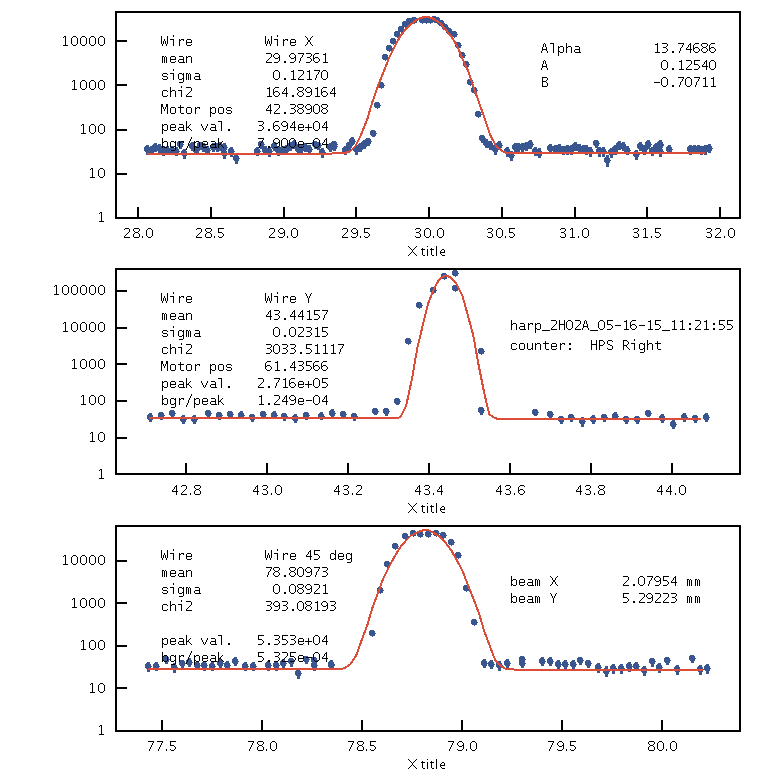
\includegraphics[width=1.0\textwidth]{pics/experiment/harpScan.png}
  \caption[Beam profile from harp scan during 2015 run]{Harp scan showing the beam profile during May 2015 running. This particular harp scan is in the Hall B logbook, entry 3341231. The beam line profile in this scan is 122$\mu$m wide in $x$ by 23$\mu$m in $y$.}
  \label{Figure:harpScan}
\end{figure}

The tagger magnet as depicted in Fig.~\ref{Figure:hallB} was used for initial beam tuning from the accelerator before sending the beam through to the HPS detectors. By energizing the tagger magnet, the electron beam was visible at the tagger dump viewer and could be aligned at the center of the viewer. Before sending the beam to HPS, harp scans were performed to measure the position and width of the beam spot~\cite{beamline_nim_2017}. Once the harp scans showed the beam to be of an acceptable size and position upstream of HPS, the tagger magnet was de-gaussed for HPS running. Without the tagger magnet on, the electron beam passes through the hall to the HPS setup as shown in Fig.~\ref{Figure:hpsBeamline}. \\
\indent The HPS setup consists of a three-dipole chicane with magnetic fields in the vertical direction. The target and the SVT are housed in the central magnet known as the pair spectrometer, or analyzing magnet. The pair spectrometer has a pole length of 91.44~cm and width of 45.72~cm. For 2.2~GeV electrons, the central magnetic field of the pair spectrometer magnet is 0.5~T~\cite{beamline_nim_2017}. For other beam energies, the analyzing magnet magnetic field is scaled accordingly. In the Engineering Run in May 2015, with a beam energy of 1.056~GeV, the pair spectrometer had a central field value of 0.24~T. The Frascati magnets, one on each side of the analyzing magnet, have magnetic fields opposite to that of the analyzing magnet such that the integrated field value over the length of the pole value of each Frascati is half of the integrated field value of the analyzing magnet. This ensures that the beam will end at the same location whether the chicane is energized or not and that the trajectory of beam energy electrons in the magnetic field is consistent across different beam energies. The magnetic field of the HPS beam line in the chicane is shown in Fig.~\ref{Figure:bField}.\\
\indent The magnetic fields of the magnets were carefully measured and mapped. The trajectory of particles was studied using these magnetic field maps that included fringe field effects. The position of the pair spectrometer magnet with respect to the Frascati magnets was optimized from these field mappings. The horizontal trajectory of a beam energy electron is shown in Fig.~\ref{Figure:trajectory}.\\
\indent In Fig.~\ref{Figure:trajectory}, the target position is where the $z$ position is zero. The entry angle of the beam at the target was determined to be approximately 30.5~mrad. At 70~cm from the target, the pair spectrometer magnet and vacuum chamber are centered on the position of the photon trajectory from the target such that the photons pass unobstructed through all subsequent vacuum chambers. The pair spectrometer magnet was placed 8.87~cm beam left, thus placing the HPS target position 2.14~cm to the right of the magnet center line. By modeling the vacuum chambers and magnetic fields in the GEant4 Monte Carlo (GEMC) framework, the particle trajectories through the HPS beam line can be observed as in Fig.~\ref{Figure:gemc}.\\
\indent As shown in ~\ref{Figure:gemc}, the beam energy electrons clearly pass through the exit hole of the last vacuum chamber (contained in the second Frascati dipole) and continue traveling to the Faraday cup where the beam charge can be measured. The beam line was modeled in GEMC and, in real running, utilized a multitude of monitors to ensure clear passage of the beam.\\
\indent The passage of the beam through the HPS beam line was monitored using beam position monitors (BPMs), wire scans with halo counters, beam viewers, and a Faraday cup. The three upstream nA BPMs give continuous beam current and position readings. These BPMs can indicate that the beam is scraping the beam pipe when the current readings fluctuate and differ with respect to each other. The current readings from the BPMs were compared to the current reading at the Faraday Cup (located downstream of the HPS beam line at the dump). When the beam current is at 50~nA or below, the reading at the Faraday Cup current is roughly the same as the current read out by the upstream BPMs and indicates no beam scraping in the beam pipe. When operating at currents above 50~nA, it was standard to insert a beam blocker in front of the Faraday Cup in order to protect it. The beam stopper would then create an offset in the Faraday Cup current readout and the actual beam current. Additionally, a fluorescent viewer screen at the Faraday Cup was used to show the beam position.  A video camera streaming a view of the screen was used for remotely observing the relative beam position on the screen. \\ 
\indent Harp scans measure the current and position of the beam through interaction with the beam (as compared to the passive, continuous readout employed through the BPMs). A harp scan moves wires through the beam vertically, horizontally, and diagonally while  downstream halo counters measure the scattered beam electron spray. The halo counters are photomultiplier tubes (PMT) strapped around the beam pipe line. The intensity of the electron spray detected by the PMTs is proportional to the beam charge that the wire interacts with. A typical harp scan from the Engineering Run is shown in Fig.~\ref{Figure:harpScan}.\\
\indent The beam profile is narrower in $y$ (vertically) than in $x$ (horizontally). The proposed beam profile for the HPS experiment was 50~$\mu$m in $y$ and 300~$\mu$m in $x$ in order to prevent overheating at the target and allow for precise vertex reconstruction. While overheating was not a limiting factor in the experiment, most of the 2015 running had a beam profile of no larger than 50~$\mu$m in $y$ and 150~$\mu$m in $x$. 

\subsection{Beam line protection}
The SVT is ideally as close to the beam as possible in order to maximize acceptance for heavy photons. The nominal SVT position has the first layer of the SVT at $\pm0.5$~mm from the active beam. Passive and active measures were employed during experimental running to prevent damage to the silicon if the beam position or quality changes during running. The collimator is a 1~cm thick tungsten plate placed upstream of the SVT with slit through which the beam can pass. A collimator prevents direct damage to the silicon should the beam move vertically from its nominal position by absorbing the beam. For the Engineering Run, the 4~mm slit width was used. \\
\indent The active beam line protection element is the Fast Shut Down (FSD) system.The FSD, when triggered, is capable of shutting of the electron beam from the injector in 1~ms. HPS used the halo counters closest to the HPS experiment to trigger the FSD in events when the beam shifted or the quality deteriorated, significantly. When the beam shifted vertically, it would first hit the inactive region of the SVT silicon sensors and scatter, increasing the rates in the halo counters. When the rates surpassed a pre-determined threshold, the FSD was tripped. If the beam hit the collimator, this also increased the rates in the halo counters and tripped the FSD. 

\subsection{Target}

The primary HPS target is a thin tungsten foil that is mounted on a support frame that can be fully retracted from the beam when not in use. For 1.1~GeV and 2.2~GeV running, the design thickness of the target tungsten foil is 0.125$\%$ radiation lengths (approximately 4~$\mu$m). The measured thickness of the actual target was 0.116$\%$. There is also a tungsten target of 0.25$\%$ radiation lengths for future running at 4.4~GeV and 6.6~GeV. The target support frame inserts the foil target from above the beam using a stepping motor linear actuator. The bottom of the target foil is free-standing so that the target can be inserted into the active beam without interruption.   
